\section{Implementazione del codice in C++}
Per la risoluzione di leggi di conservazione non lineari 2D su griglie triangolari è stata sviluppata la libreria \texttt{ConservationLaw2D}, in gran parte scritta in C++.

Il codice permette di risolvere problemi basati su diversi tipi di modelli, con particolar riguardo alle equazioni di Eulero 2D. Non mancano però esempi sulle equazioni dell'acustica o di onde in acque basse. Inoltre è possibile estendere il codice ad altri modelli o metodi di risoluzione (come Discontinous Galerkin) con relativa semplicità.

La struttura del codice si organizza essenzialmente su in tre parti distinte:
\begin{enumerate}
\item La gestione della mesh;
\item La descrizione del modello (Eulero ad esempio);
\item Il solutore (Volumi Finiti).
\end{enumerate}

\subsection{La gestione della mesh}
La parte più sostanziosa e certamente meno banale è quella riguardante la gestione della mesh. 

Il requisito essenziale nel nostro caso riguarda la possibilità di effettuare particolari ``query'' sulle relazioni tra i vari elementi. Questo tipo di problema può essere risolto in svariati modi, ma ognuno è un compromesso tra utilizzo di memoria ed efficienza.

Ad esempio, alcuni tipi di query possono essere:
\begin{itemize}
\item Dato un vertice, quali sono i poligoni ad esso adiacenti, ossia quali poligoni hanno tra i propri vertici quello in questione? 
\item Dato un poligono, quali sono i poligoni ad esso adiacenti, cioé che condividono con esso un lato? 
\item Dato un lato, quali sono i poligoni che insistono su di esso? 
\end{itemize}

Gli oggetti che compongo una mesh sono gli elementi, i lati e i vertici. Ognuno è collegato all'altro secondo relazioni di appartenenza, per esempio un lato è formato da due vertici, e un poligono è un insieme di lati. Quindi se volessi sapere quali sono i vertici del poligono basterebbe scorrere sui lati e restituire i vertici. Già in questo caso molto semplice però vi sono difficoltà: il lato non è in genere orientato, quindi quale dei due vertici considerare? Un triangolo ha 3 lati, quindi dei 6 vertici forniti da questi ultimi 3 saranno coincidenti, ma non è a priori stabilita una regola per recuperare una lista di vertici unici (magari anche in ordine antiorario).

Sono inoltre molto complesse (e quindi dispendiose in termini computazionali) query che devono risolversi in ordine inverso, per esempio recuperare i poligoni adiacenti ad un vertice. In teoria dovrei scorrere tutti i poligoni della mesh e per ognuno scorrere i vertici, e fare poi un confronto.

Riassumendo dunque, cerchiamo una struttura dati che non soffra troppo nella risoluzione di query di adiacenza, che fornisca un certo orientamento ai lati e che magari non sia dispendiosa in termini di memoria.

La struttura dati che abbiamo deciso di adottare è di tipo \emph{half-edge}, dove ogni lato è memorizzato come coppia di lati gemelli orientati però in direzioni opposte. In particolare, ogni elemento è descritto da una successione in senso antiorario di half-edge, ognuno dei quali ha un puntatore al suo successivo, al vertice di origine, all'elemento alla sua sinistra (ricordiamo che il segmento è orientato) e al suo lato gemello (se esiste), appartenente all'elemento adiacente a quel lato. Una mesh di questo tipo è detta \emph{edge-based}\footnote{Le mesh basate su half-edge sono spesso utilizzate nella Computer Grafica perché permettono anche di descrivere superficie tridimensionali. Non è però l'unica possibilità esistente, anzi ve ne sono molte altre (winged-edge, quad-edge).}.

La scelta di utilizzare questa struttura dati fornisce qualcosa che non è troppo oneroso in termini di memoria, sufficientemente efficiente e abbastanza robusto nell'eventualità di una futura estensione a tecniche di raffinamento e deraffinamento, le quali eliminando triangoli possono rendere difficoltoso l'aggiornamento della struttura delle adiacenze.

Le query anche complesse in questa topologia diventano molto semplici ed intuitive: 
\begin{itemize}
\item I vertici di un poligono si trovano partendo da un suo mezzo lato qualsiasi, restituendo il vertice di quest'ultimo per poi passare al mezzo-lato successivo, e da qui ripetere; 
\item Il poligono adiacente ad un mezzo-lato dato, che è il poligono del lato gemello al lato dato;
\end{itemize}
Non mancano però le difficoltà, infatti questa struttura dati deve essere modificata in presenza di bordi o di vertici degeneri (un vertice è degenere se è in comune a due poligoni i quali però non hanno lati in comune tra loro, come il nodo di un papillion).

La seconda scelta progettuale di rilevanza riguarda invece la possibilità di utilizzare mesh composte da poligoni di un numero di lati non necessariamente identico (quindi non necessariamente triangolari): i Volumi Finiti infatti si applicano perfettamente a prescindere dal numero di lati del volume di controllo. La struttura dati utilizzata ha permesso di implementare tale scelta senza grossi sforzi aggiuntivi.

Infine una terza importante caratteristica è la possibilità di estendere le classi che descrivono vertice, lato e poligono a proprio piacimento, senza influenzare però la struttura dati. La mesh può quindi essere puramente topologica (essenzialmente un grafo), oppure avere anche una struttura geometrica o, come nel nostro caso, una struttura di spazio funzionale, dove ogni poligono descrive anche una funzione costante (e dunque la mesh descrive una funzione costante a tratti). In questo ambito si è fatto ricorso ad un uso moderato di \emph{templates}.
\subsubsection{La struttura dati half-edge}
Iniziamo con il descrivere dettagliatamente la struttura dati utilizzata. Come accennato, la struttura dati half-edge è di tipo edge-based, quindi gran parte dell'informazione strutturale è associata ai lati.

\begin{figure}[htb]
\centering
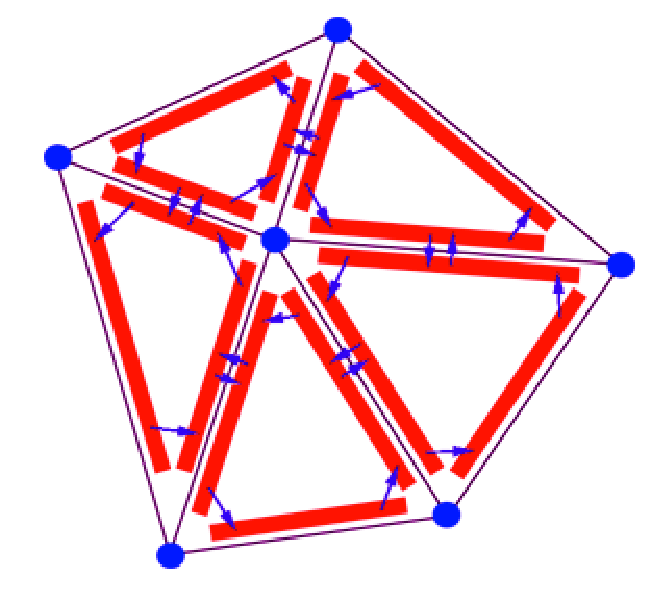
\includegraphics[width=5.8cm]{images/halfedge.pdf}
\caption{Struttura dati di tipo half-edge} \label{fig:halfedge}
\end{figure}

In Figura \ref{fig:halfedge} è rappresentato il patch di elementi di un vertice, con le relazioni esistenti tra i vari lati. L'orientamento predefinito dei lati è in senso antiorario, come si evince seguendo il senso delle frecce.

Oltre a questi puntatori, per descrivere la mesh è necessario collegare ai lati i vertici e i poligoni. Ogni vertice ha un puntatore ad uno dei lati\footnote{Come sarà spiegato più avanti, questo è in realtà falso perché sono necessarie delle modifiche per poter gestire i vertici di bordo.} che esce da esso (e viceversa ogni lato ha un puntatore al vertice d'origine), e ogni poligono ha un puntatore ad uno qualsiasi dei suoi lati (e anche in questo caso, ogni lato ha un puntatore al poligono alla sua sinistra).

Nel codice sono state definite 5 classi primitive per la struttura dati:
\begin{itemize}
\item \texttt{BaseKernel}, contenitore di tipi di dati ereditato da tutte le classi;
\item \texttt{BaseVertex}, la classe basilare del vertice, che contiene le coordinate e un puntatore ad un halfedge che da esso parte;
\item \texttt{BaseHEdge}, la classe che descrive l'halfedge, con puntatori al vertice di partenza, al lato successivo, a quello gemello e anche un puntatore al poligono alla sua sinistra. Vi sono poi metodi per accedere ai due vertici e ai due poligoni adiacenti (sempre se quello a destra esiste);
\item \texttt{BasePolygon}, la classe che descrive il poligono, contiene un puntatore ad uno dei suoi lati;
\item \texttt{BasePolygonalMesh}, ossia la mesh vera e propria che mette a disposizione iteratori sui suoi elementi (contenuti in tre liste, una per i vertici, una per i lati e una per i poligoni), nonché metodi per aggiungere nuovi poligoni e vertici.
\end{itemize}
Inoltre sia i lati che i poligoni hanno un attributo \texttt{color}, come fosse un marker che ci permette di distinguerli. Ad esempio questo ci permette di assegnare un certo valore di soluzione solo ad alcuni poligoni che abbiamo precedentemente marcato, e stessa cosa per i lati (utile nell'assegnazione delle condizioni iniziali e di bordo).
 
Tutte queste classi hanno il prefisso \texttt{Base} perché devono essere necessariamente estese, eventualmente da classi vuote (che con molta fantasia chiameremo allo stesso modo, senza il prefisso). Questo passaggio a prima vista fittizio sarà giustificato in seguito.
\paragraph{Il caso dei vertici degeneri}
Consideriamo una mesh composta da soli due triangoli i quali condividono un solo vertice. In questo caso la struttura dati non riesce a rappresentare la mesh perché partendo dal vertice e seguendo il suo puntatore ad uno dei due half-edge rimaniamo ``intrappolati'' sul triangolo indicato dal lato scelto, senza possibilità di passare a quello adiacente. In questo caso si parla di vertice degenere.

Per ovviare al problema abbiamo studiato una soluzione possibile, che per quanto macchinosa mantiene comunque tempi ragionevoli di accesso. 

L'idea è quella di salvare nel vertice la lista dei lati (e non solo uno) che si irradiano da esso. Però non è necessario avere un puntatore ad ognuno, piuttosto basta avere un puntatore ai soli lati di bordo e nell'eventualità che il vertice sia interno ad un solo lato qualsiasi.
La struttura dunque è ridondante solo nelle situazioni particolari.

\subsubsection{I circolatori}
La struttura dati descritta introduce in modo naturale il concetto di \emph{circolatore}.

È evidente ad esempio che la lista dei vertici di un poligono non ha testa né coda. Quindi partendo da un qualsiasi vertice dovrebbe essere possibile passare a quello subito successivo o precedente, eventualmente tornando su sé stesso dopo un giro completo. Pensando più in prospettiva si può quindi immaginare che anche la risposta di una query di adiacenza sia un circolatore.

Un esempio pratico di utilizzo dei circolatori è il seguente, dove per ogni vertice viene calcolata l'area media dei poligoni adiacenti.

Iniziamo con l'intestazione del codice, dove viene definito il circolatore:
\begin{lstlisting}[name=esempioCirc]
#include <mesh/mesh_default_traits.hpp>

using namespace ConservationLaw2D;

typedef Mesh::DefaultTraits<double> Traits;
typedef Traits::PolygonalMesh       SimpleMesh;

typedef SimpleMesh::vertex_it                  v_it;
typedef SimpleMesh::Vertex::PolygonCirculator  vp_cit;
\end{lstlisting}
Di seguito riportiamo invece il blocco principale:
\begin{lstlisting}[name=esempioCirc]
// Itero su tutti i vertici della mesh
for ( v_it v = mesh.v_begin(); v != mesh.v_end(); ++v ) {
    // Contatore per il numero di poligoni adiacenti
    size_t count(0);
    real_t tmparea(0.0);
    // Inizializzo il circolatore
    vp_cit p = (*v)->beginP();
    do {
        tmparea += p->area();
        count++;
        // Incremento il circolatore ...
        p++;
    // ... finche' non torno al punto di partenza
    } while( p != (*v)->beginP() );
    cout << tmparea/count << endl;
}
\end{lstlisting}
Come si può osservare una query relativamente complessa come il trovare i poligoni adiacenti al vertice dato si può scrivere con poche righe di codice, mantenendo allo stesso tempo un buon livello di astrazione. Allo stesso modo si possono trovare i lati o i vertici adiacenti al vertice dato (con i circolatori \texttt{Vertex::HEdgeCirculator} e \texttt{Vertex::VertexCirculator}). Oppure, dato un poligono, si possono cercare vertici, lati e poligoni adiacenti (rispettivamente con i circolatori \texttt{Polygon::VertexCirculator}, \texttt{Polygon::HEdgeCirculator} e \texttt{Polygon::PolygonCirculator}).

Il circolatore è definito attraverso un'unica classe \texttt{CirculatorTS}, specializzata poi attraverso l'uso di template. Si tratta di una classe generica dalla quale sono derivati tutti i circolatori possibili (escludendo quelli riferiti ai lati sono esattamente 6, elencati subito sopra). In questo modo a costo di un livello di astrazione e complessità maggiore si ha un codice molto più compatto.

La specializzazione di un circolatore avviene con una definizione del tipo (all'interno della classe \texttt{BaseVertex}):
\begin{lstlisting}
typedef typename Circulators::CirculatorTS<KERNEL,Polygon,Vertex>  PolygonCirculator;
\end{lstlisting}
dove viene definito un circolatore sui poligoni adiacenti al vertice dato. In questo modo la classe automaticamente selezionerà i metodi opportuni per circolare sui poligoni partendo da un vertice\footnote{Non essendo possibile la specializzazione parziale questa selezione avviene tramite delle variabili \emph{dummy}, una di tipo \texttt{T} e una di tipo \texttt{S} (per esempio \texttt{Polygon} e \texttt{Vertex}). I metodi necessari alla specializzazione sono quindi selezionati per overloading.}.

Essenzialmente le due procedure principali riguardando l'incremento del circolatore (cioè il passaggio all'elemento successivo) e la lettura dell'elemento corrente. Tutti i circolatori infatti non hanno un puntatore all'oggetto corrente, bensì un puntatore ad un particolare half-edge dal quale si risolve facilmente l'elemento corrente.

Sempre considerando il circolatore prima definito, la procedura di lettura ha la forma seguente:
\begin{lstlisting}
return current_hedge->polygonL();
\end{lstlisting}
quindi \texttt{current\_hedge} è semplicemente un lato del poligono corrente.

La procedura di incremento è invece più complessa:
\begin{lstlisting}
typedef typename KERNEL::HEdge_ptr hedge_ptr;
hedge_ptr tmphe(current_hedge);
do {
    current_hedge = &(current_hedge->getNextHEdge());
} while ( &(current_hedge->getNextHEdge()) != tmphe);
if ( current_hedge->isBoundary() ) {
    // Halfedge di bordo
    current_vertex_hedge = (current_vertex_hedge+1) % hedges->size();
    current_hedge = (*hedges)[current_vertex_hedge];
} else {
    // Tutto regolare
    current_hedge = &(current_hedge->getTwinHEdge());
}
\end{lstlisting}
Il primo blocco \texttt{do} cerca semplicemente l'halfedge precedente, girando intorno al poligono. Nel secondo blocco \texttt{if} invece si controlla se il lato trovato è di bordo o no: nel secondo caso, più immediato, viene semplicemente restituito un puntatore all'halfedge gemello, che avrà alla sua sinistra il poligono adiacente (ciò che cercavamo). Nel secondo caso invece si dovrebbe tornare al punto di partenza (cioè all'halfedge che ha inizializzato il circolatore), però si deve fare attenzione al caso di vertici degeneri. Quindi nel circolatore è tenuta in memoria una lista dei lati di bordo del vertice, in modo che si passi semplicemente al successivo.
 
La procedura opera sempre in senso antiorario, e questo è garantito anche se il vertice è al bordo o è degenere.
\subsubsection{La costruzione della struttura dati}
La parte più complessa della struttura dati è la procedura atta a riempirla (e probabilmente la più complessa dell'intero codice). Questo perché l'algoritmo deve essere efficiente e allo stesso tempo deve permettere di costruire la mesh in modo incrementale, aggiungendo un elemento alla volta.

Per costruire una mesh si inizia aggiungendo i vertici. Ad esempio:
\begin{lstlisting}[name=esempioMesh]
vector<vertex_ptr> vhandle;
vhandle.reserve(4);
vhandle[0] = mesh.addVertex(0, 0);
vhandle[1] = mesh.addVertex(1, 0);
vhandle[2] = mesh.addVertex(0, 1);
vhandle[3] = mesh.addVertex(1, 1);
\end{lstlisting}
Una volta che sono disponibili dei puntatori a vertici, si aggiungono i poligoni:
\begin{lstlisting}[name=esempioMesh]
vector<vertex_ptr> poly_vertex;
poly_vertex.reserve(3);
poly_vertex.push_back( vhandle[0] );
poly_vertex.push_back( vhandle[1] );
poly_vertex.push_back( vhandle[2] );
mesh.addPolygon( poly_vertex );

poly_vertex.clear();
vector<vertex_ptr> poly_vertex;
poly_vertex.reserve(3);
poly_vertex.push_back( vhandle[0] );
poly_vertex.push_back( vhandle[2] );
poly_vertex.push_back( vhandle[3] );
mesh.addPolygon( poly_vertex );
\end{lstlisting}
Analizziamo più approfonditamente la procedura \texttt{addPolygon}.

Iniziamo con il creare un puntatore ad un poligono:
\begin{lstlisting}[name=addPolygon]
// Creo il poligono
polygon_ptr poly( new Polygon() );
\end{lstlisting}
A questo punto creiamo i lati impostando per ognuno il poligono corrispondente (ossia quello che stiamo creando) e il vertice iniziale.
\begin{lstlisting}[name=addPolygon]
// Creo i lati del poligono
size_t nsides = v.size();
// Se aggiungo un triangolo e la mesh e' triangolare rimane triangolare
isTriangular_ &= (nsides == 3);
vector<hedge_ptr> he(nsides);
for (size_t i = 0; i < nsides; ++i) {
    // Nuovo halfhedge
    he[i] = (hedge_ptr)new HEdge();
    // Imposto il poligono a sinistra del lato
    he[i]->polygon_ = poly;
    // Imposto il vertice iniziale
    he[i]->vertex_ = v[i];
    // Aggiungo alla lista dei lati
    hedges_.push_back(he[i]);
}
\end{lstlisting}
Adesso facciamo in modo che il poligono punti ad uno dei lati appena creati (per esempio il primo):
\begin{lstlisting}[name=addPolygon]
// Aggiungo al poligono uno dei suoi lati
poly->hedge_ = he[0];
\end{lstlisting}
Adesso dobbiamo costruire i collegamenti tra gli halfedge (sia tra quelli creati che tra quelli già presenti). Si inizia impostando il successivo di ognuno, e si procede verificando se il vertice di partenza è nuovo oppure è già presente.

Nel primo caso devo cercare l'halfedge gemello, e sarà quello che nella lista dei lati adiacenti al vertice avrà come vertice il vertice di arrivo del lato in esame. Si fa quindi ricorso al circolatore sui lati.

Nel secondo caso invece per il momento non faccio nulla (questo sarà infatti un lato di bordo e merita particolari attenzioni). 
\begin{lstlisting}[name=addPolygon]
// Collegamenti tra halfedge
typedef typename Vertex::HEdgeCirculator HECirc;
for (size_t i = 0; i < nsides; ++i) {
    // Imposto il successivo
    he[i]->nexthedge_ = he[(i+1)%nsides];
    // Verifico se il vertice corrispondente e' nuovo
    if ( v[i]->hedges_.size() != 0 ) {
        // Gia' presente, cerco eventuali collegamenti
        HECirc vhec = v[i]->beginE();
        bool found = false;
        do {
            ++vhec;
            found = ( vhec->vertex_ == v[(i+1)%nsides]);
        } while(!found && vhec != v[i]->beginE());
        if (found) {
            // Trovata corrispondenza, salvo
            he[i]->twinhedge_ = &(*vhec);
            poly->hedge_ = he[i];
            vhec->polygon_->hedge_ = &(*vhec);
        }
    }
}
\end{lstlisting}
Adesso aggiungiamo i lati alla mesh e al vertice corrispondente:
\begin{lstlisting}[name=addPolygon]
// Collego il nuovo elemento con la mesh
for (size_t i = 0; i < nsides; ++i) {
    v[i]->hedges_.push_back(he[i]);
    if ( he[i]->twinhedge_ ) {
        he[i]->twinhedge_->twinhedge_ = he[i];
    }
}
\end{lstlisting}
Ora dobbiamo aggiornare la struttura dati dei vertici, in modo tale da permette ai circolatori di gestire i casi di bordo. Nella lista sono già presenti tutti lati precedentemente aggiunti (che sono tutti di bordo) insieme a quelli aggiunti adesso, che invece possono essere interni. L'idea è quella di scorrerli tutti e rimuovere quelli che non sono più di bordo. Se non dovesse rimanere nulla aggiungo allora un lato caso tra quelli che erano presenti (in questo caso il vertice diventa interno).
\begin{lstlisting}[name=addPolygon]
// Aggiorno la struttura dati dei vertici
typedef typename vector<hedge_ptr>::iterator Iterator;
for (size_t i = 0; i < nsides; ++i) {
    Iterator it = v[i]->hedges_.begin();
    while ( it != v[i]->hedges_.end() ) {
        if ( !(*it)->isBoundary() ) {
            it = v[i]->hedges_.erase( it );
        } else {
            ++it;
        }
    }
    // Se e' vuoto ne metto uno a caso
    if ( v[i]->hedges_.empty() ) {
        v[i]->hedges_.push_back(he[i]);
    }
}
\end{lstlisting}
Infine inseriamo il poligono nella lista della mesh:
\begin{lstlisting}[name=addPolygon]
// Aggiungo il poligono alla mesh
polygons_.push_back(poly);
\end{lstlisting}

Nel codice è anche presente una procedura (\texttt{Mesh::IO::MeshReader}) in grado di leggere da file una mesh.
\subsubsection{Traits della Mesh}
La struttura dati che gestisce la mesh è composta da vertici, lati ed elementi poligonali. Estendere però queste classi può diventare difficoltoso perché sono intimamente legate tra loro, per via della struttura topologica. Una possibile soluzione è quella di utilizzare i templates e definire le classi solo una volta che sono state estese.

Supponiamo ad esempio di aver definito le classi primitive \texttt{BaseVertex}, \texttt{BaseHEdge}, \texttt{BasePolygon} e \texttt{BasePolygonalMesh}. Queste non sono ancora ben definite, ma dipendono dalla scelta del \texttt{KERNEL}.

Si procede allora in questo modo:
\begin{lstlisting}
template <typename T>
struct DefaultTraits {
    class Kernel;
    class Vertex;
    class HEdge;
    class Polygon;
    class PolygonalMesh;
           
    class Kernel : public BaseKernel<T, Vertex, HEdge, Polygon, PolygonalMesh> {};
    class Vertex : public BaseVertex<Kernel> {};
    class HEdge : public BaseHEdge<Kernel> {};
    class Polygon : public BasePolygon<Kernel> {};
    class PolygonalMesh : public BasePolygonalMesh<Kernel> {};
};
\end{lstlisting}
Per esempio la classe \texttt{Vertex} deriva dalla classe \texttt{BaseVertex}, la quale però ha come parametro \texttt{KERNEL}, che a sua volta dipende da \texttt{Vertex} stesso! In realtà il cane non si morde la coda, perché il compilatore si fida del fatto che la classe Vertex verrà definita in seguito. In questo modo un metodo della classe \texttt{BaseVertex} (e quindi della classe \texttt{Vertex}) può restituire un tipo di dato \texttt{Vertex} senza dover complicare troppo il codice con metodi virtuali.

La classe \texttt{BaseKernel} mette a disposizione dei tipi comuni a tutte le altri classi\footnote{In questo modo, ad esempio, se si volessero utilizzare \emph{smart pointer} si dovrebbe cambiare solo questa classe.}:
\begin{lstlisting}
template 
<typename RTYPE, typename VERTEX, typename HEDGE, typename POLYGON, typename MESH>
struct BaseKernel {
    typedef RTYPE     real_t;
    typedef VERTEX    Vertex;
    typedef HEDGE     HEdge;
    typedef POLYGON   Polygon;
    typedef MESH      Mesh;
    typedef Vertex*   Vertex_ptr;
    typedef HEdge*    HEdge_ptr;
    typedef Polygon*  Polygon_ptr;
};
\end{lstlisting}

In questo modo è possibile estendere a proprio piacimento le classi della mesh senza dover intervenire sulle classi primitive. Nel caso dei Volumi Finiti per esempio si potrebbe avere:
\begin{lstlisting}
template <typename T, typename SOLTYPE>
struct DefaultTraits {
    class Kernel;
    class Vertex;
    class HEdge;
    class Polygon;
    class PolygonalMesh;

    class Kernel : public BaseKernel<T, Vertex, HEdge, Polygon, PolygonalMesh> {};
    class Vertex : public BaseVertex<Kernel> {};
    class HEdge : public BaseHEdge<Kernel> {};
    class Polygon : public BasePolygon<Kernel> {
        public:
            SOLTYPE sol, sol0;
    };
    class PolygonalMesh : public BasePolygonalMesh<Kernel> {};
};
\end{lstlisting}
In questo caso abbiamo esteso la classe \texttt{Polygon} aggiungendo due attributi \texttt{sol} e \texttt{sol0}, che rappresentano la soluzione in quel dato elemento (in generale sono dei vettori).

Nella realtà la specializzazione della mesh per i Volumi Finiti comprende anche altri metodi ed attributi (che non riportiamo in dettaglio in questa sede), come ad esempio la possibilità di memorizzare una volta per tutte le caratteristiche geometriche degli elementi, in modo da ottimizzare il codice in fase di esecuzione.

\subsection{La struttura del solutore a Volumi Finiti}
Una volta che si ha a disposizione una struttura sufficientemente robusta per gestire la mesh, scrivere un solutore a Volumi Finiti diventa relativamente semplice, in quanto l'algoritmo \eqref{eq:schemavolumifiniti} non presenta particolari complessità di implementazione.

Il nostro obiettivo però è stato quello di scrivere una classe che fosse compatibile con diversi modelli e diversi flussi numerici. Infatti si può osservare che questi termini entrano in gioco solo nel calcolo del termine ``di destra'' dello schema numerico: questo dipende dal flusso numerico, il quale a sua volta dipende dal modello in esame.

Vediamo quindi la struttura generale della classe \texttt{Solver::FiniteVolume}:
\begin{lstlisting}
template <typename MODEL, typename NUMFLUX>
class FiniteVolume {
	private:
		typedef typename MODEL::real_t							real_t;
		typedef typename MODEL::SolType							SolType;
		typedef typename Mesh::DefaultTraits<real_t,SolType>	Traits;
	public:
		// Mesh
		typedef typename Traits::PolygonalMesh		FVMesh;
	private:
		// Condizioni iniziali e termine sorgente
		// [in ingresso x, y e colore]
		typedef SolType (*INITCOND)( size_t, real_t, real_t );
		// [in ingresso stato a sinistra, x, y, normale, t e colore]
		typedef SolType (*BOUNDARYCOND)( SolType&, size_t, real_t, real_t, real_t, real_t, real_t );
		// [in ingresso x, y, t e colore]
		typedef SolType (*SOURCE)( const SolType&, size_t, real_t, real_t, real_t );

		// Valuta rhs del poligono dato
		inline SolType RHS( const polygon_ptr ) const;

	public:
		FiniteVolume( MODEL& model, FVMesh& mesh )
			:model_(model),mesh_(mesh),NumFlux(model),cflmax_(0.0),hmax_(0.0),currtime_(0.0) {};
		
		// Impostazioni
		void setCFLmax ( real_t cflm ) { cflmax_ = cflm; }
		void setIC ( INITCOND ic ) { InitialCondition = ic; }
		void setBC ( BOUNDARYCOND bc ) { BoundaryCondition = bc; }
		void setSource ( SOURCE s ) { Source = s; }
		void setDirectory ( const string& dir ) { datadir_ = dir; }
		// Accesso
		real_t getCurrTime(void) { return currtime_; }
		real_t getCurrDt(void) { return dt_; }
		
		// Inizializza il solutore
		void init();
		// Passo temporale
		void timestep();
	private:
		void updateTimestep();
	public:
		void framegrab(size_t const, bool, bool) const;

	private:
		// Modello
		MODEL& model_;
		// Mesh
		FVMesh& mesh_;
		// Flusso numerico
		NUMFLUX NumFlux;
		// Condizioni iniziali e bordo
		INITCOND		InitialCondition;
		BOUNDARYCOND	BoundaryCondition;
		SOURCE			Source;
		// Altro
		real_t cflmax_, hmax_, dt_, currtime_;
		string datadir_;
};
\end{lstlisting}
La definizione della classe dipende da due parametri, il flusso numerico \texttt{NUMFLUX} e il modello \texttt{MODEL}. La mesh è definita all'interno del solutore, in modo che possano essere disponibili le estensioni necessarie (linea 9).

Per le condizioni iniziali, al bordo e il termine sorgente sono definite le signature delle funzioni che il codice principale dovrà fornire. Osserviamo che le funzioni hanno tra i parametri d'ingresso il colore dell'oggetto in esame (per esempio poligono o lato): in questo modo diventa molto semplice assegnare condizioni al contorno solo su alcune porzioni di bordo oppure imporre il termine sorgente solo all'interno di un sottodominio.

Tra i metodi pubblici del solutore vi sono quelli atti ad assegnare tutti i parametri necessari alla simulazione, come il numero CFL massimo o la directory nella quale salvare i risultati dell'elaborazione.

Il metodo più importante, che analizziamo in dettaglio, riguarda invece l'esecuzione di un passo temporale. Questo non è nient'altro che l'implementazione dello schema a Volumi Finiti:
\begin{lstlisting}
template <typename MODEL, typename NUMFLUX>
inline void FiniteVolume<MODEL,NUMFLUX>::timestep( void ) {
	// Salvo la soluzione al passo precedente e calcolo maxLambda
	updateTimestep();
	for (p_it p = mesh_.p_begin(); p != mesh_.p_end(); ++p) {
		(*p)->sol0 = (*p)->sol;
		if ( !model_.ConsistentState((*p)->sol0) ) {
			std::cerr << "Bad state solution! Maybe too high CFL number ..." << std::endl;
			exit(1);
		}
	}
	// Itero sui poligoni
	for (p_it p = mesh_.p_begin(); p != mesh_.p_end(); ++p) {
		// Risolvo l'ODE
		(*p)->sol = (*p)->sol0 + dt_ * RHS(*p);
	}
	// Aggiorno currtime_
	currtime_ += dt_;
}		
\end{lstlisting}
Il codice si commenta da solo: nella prima parte si aggiorna il passo temporale e si controlla la consistenza della soluzione (per esempio pressioni o densità negative), mentre nella seconda parte si esegue il passo temporale. In questa parte tutto il calcolo vero e proprio è delegato alla procedure \texttt{RHS}:
\begin{lstlisting}
template <typename MODEL,typename NUMFLUX>
inline typename MODEL::SolType FiniteVolume<MODEL,NUMFLUX>::RHS( const polygon_ptr p ) const {
	// Valuto il flusso attraverso i bordi
	SolType Flux = SolType::Zero();
	// Stato a sinistra
	SolType qlstate = p->sol0;
	// Stato a destra
	SolType qrstate;
	he_cit e = p->beginE();
	do {
		if ( !e->isBoundary() ) {
			// Lato interno
			qrstate = e->polygonR().sol0;
		} else {
			// Lato di bordo
			SolType wl = model_.ConservativeToPrimitive(qlstate);
			SolType wr = BoundaryCondition(wl,e->getColor(),e->xm(),e->ym(),e->nx(),e->ny(),currtime_);
			qrstate = model_.PrimitiveToConservative(wr);
		}
		Flux += e->length() * NumFlux(qlstate, qrstate, e->nx(), e->ny());
		++e;
	} while ( e != p->beginE() );
	// Valuto il termine sorgente, se presente
	SolType SourceTerm = SolType::Zero();
	if ( !Source ) SourceTerm = Source( qlstate, p->getColor(), p->cx(), p->cy(), currtime_ );
	// Sommo e divido per l'area
	return (SourceTerm - Flux) / p->area();
}
\end{lstlisting}
Il nodo cruciale della procedura precedente è la distinzione tra i lati di bordo e lati interni. Nel primo caso si richiama la condizione al contorno relativa a tale lato e si assegna al poligono adiacente la condizione stessa, mentre nel secondo si utilizza il vero valore della soluzione del poligono adiacente. Una volta che si hanno a disposizione gli stati destro e sinistro del lato si può calcolare il flusso numerico.

Vi è inoltre la procedura \texttt{framegrab} (la quale, ironia della sorte, è la più lunga e complessa del solutore) il cui compito è quello di salvare su file la soluzione al passo temporale corrente, secondo il formato desiderato (Matlab o Gnuplot). Si può anche scegliere se interpolare la soluzione nei vertici (ricordiamo che la soluzione è una funzione costante a tratti ed è quindi definita solo nei baricentri dei poligoni).

\subsection{Definizione del modello e del flusso numerico}
Gli ultimi ingredienti necessari a completare la ricetta sono il modello, che deve definire metodi per il calcolo del flusso numerico esatto, degli autovalori e via discorrendo, e il flusso numerico.

Osserviamo che il flusso numerico è definito a partire dal modello (pur essendo una classe del tutto diversa): questo perché i flussi approssimati (si veda Appendice \ref{app:flussinum}), come Roe, sono definiti ad hoc per il modello in esame. Solo il flusso di Lax-Friedrichs è definito \emph{model-free}, perché necessita della sola conoscenza del flusso esatto (e del massimo autovalore locale).
\subsubsection{Il modello}
Vediamo la struttura generale di un modello (in questo caso Eulero):
\begin{lstlisting}
#define DIMENSION 4
template <typename T>
class Eulero {
	public:
		// Defininzioni vettori
		// Vettore per la soluzione
		typedef T	real_t;
		typedef Eigen::Matrix<T, DIMENSION, 1>	SolType;
		typedef Eigen::Matrix<T, DIMENSION, 2>	FluxType;
		Eulero( real_t gamma ):GAMMA(gamma) {}
		// Accesso variabili
		inline real_t R( const SolType& q ) const;
		inline real_t U( const SolType& q ) const;
		inline real_t V( const SolType& q ) const;
		inline real_t E( const SolType& q ) const;
		inline real_t P( const SolType& q ) const;
		inline real_t C( const SolType& q ) const;
		inline real_t H( const SolType& q ) const;
		inline real_t gamma(void) const;
		// Variabili primitive <-> Variabili conservate
		// [rho, u, v, p]      <-> [rho, rho u, rho v, rho e]
		inline SolType PrimitiveToConservative( const SolType& w ) const;
		inline SolType ConservativeToPrimitive( const SolType& q ) const;
		// Controlla se lo stato e' consistente
		inline bool ConsistentState( const SolType& q ) const;
		// Flusso
		inline FluxType Flux( const SolType& q );
		// Flusso in direzione normale
		inline SolType NormalFlux( const SolType& q, const real_t nx, const real_t ny ) const;
		// Massimo autovalore valutato in q
		inline real_t MaxLambda( const SolType& q );
		// Autovalori
		inline SolType EigenValues( const SolType& q, const real_t nx, const real_t ny ) const;
	private:
		real_t GAMMA;
};
\end{lstlisting}
La struttura generale del codice richiede essenzialmente la presenza di metodi per calcolare il flusso, la consistenza dello stato, il massimo autovalore e la conversione da variabili primitive a conservate. Tutti gli altri metodi elencati sono accessori.

Osserviamo infine che il tipo di dato per numeri reali è anch'esso parametrizzato, e può essere scelto proprio nella definizione del modello.

\subsubsection{Flussi numerici}
Il flusso numerico è definito infine come un funtore. Riportiamo a titolo d'esempio il flusso di Lax-Friedrichs:
\begin{lstlisting}
template <typename MODEL>
class LaxFriedrichs {
	typedef typename MODEL::real_t     real_t;
	typedef typename MODEL::SolType    SolType;
	typedef typename MODEL::FluxType   FluxType;
	public:
		LaxFriedrichs(MODEL& m):model(m) {}
		inline SolType operator()(const SolType& ql, const SolType& qr, const real_t nx, const real_t ny) const { 
			// Calcolo i flussi
			FluxType FluxL = model.Flux(ql);
			FluxType FluxR = model.Flux(qr);
			// Viscosita' artificiale
			real_t sigma = max( model.MaxLambda(ql), model.MaxLambda(qr) );
			// Flusso in direzione normale
			return 0.5 * ( (FluxL.col(0)+FluxR.col(0))*nx + (FluxL.col(1)+FluxR.col(1))*ny - sigma*(qr-ql) );
		}
	private:
		MODEL& model;
};
\end{lstlisting}
\subsection{Output dei risultati}
A margine è stata implementata una procedura che permette in modo automatico di generare l'output grafico relativo al problema studiato. In particolare vi è uno script Perl che si occupa dei processi accessori all'esecuzione vera e propria della simulazione, ad esempio pulire le directory da simulazioni precedenti o controllare che i parametri in ingresso siano corretti. Lo script si interfaccia automaticamente a GnuPlot per l'elaborazione grafica.

È possibile anche elaborare i risultati in Matlab, attraverso appositi script contenuti nella directory \texttt{tools}.

